\begin{frame}{Pêndulo amortecido}
  Considere a seguinte EDO.
  \begin{equation}\label{eq:edo-geral}
    \theta^{\prime\prime}+c\theta^{\prime}+\sen(\theta)=0,\quad c>0.
  \end{equation}
  A qual modela o pêndulo amortecido, onde $\theta$ é o angulo do pêndulo e $c$ é o amortecimento.\\
  Note que fazendo $\omega=\theta^{\prime}$, temos que a EDO \eqref{eq:edo-geral} se pode escrever como o seguinte sistema autónomo
  \begin{equation}\label{eq:edo-sistema}
    \begin{cases}
      \theta^{\prime}=\omega, \text{,} \\
      \omega^{\prime}=-\sen(\theta)-c\omega.
    \end{cases}
  \end{equation}
\end{frame}

\begin{frame}{}
  Portanto, fazendo
  \begin{align*}
    f(\theta,\omega)=\begin{pmatrix}
      \omega \\
      -\sen(\theta)-c\omega
    \end{pmatrix}=\begin{pmatrix}
      0 \\
      0
    \end{pmatrix}.
  \end{align*}
  Nos temos que $p$ é singularidade se $p=(k\pi,0)$ com $k\in\mathbb{Z}$.\\
  \begin{center}
    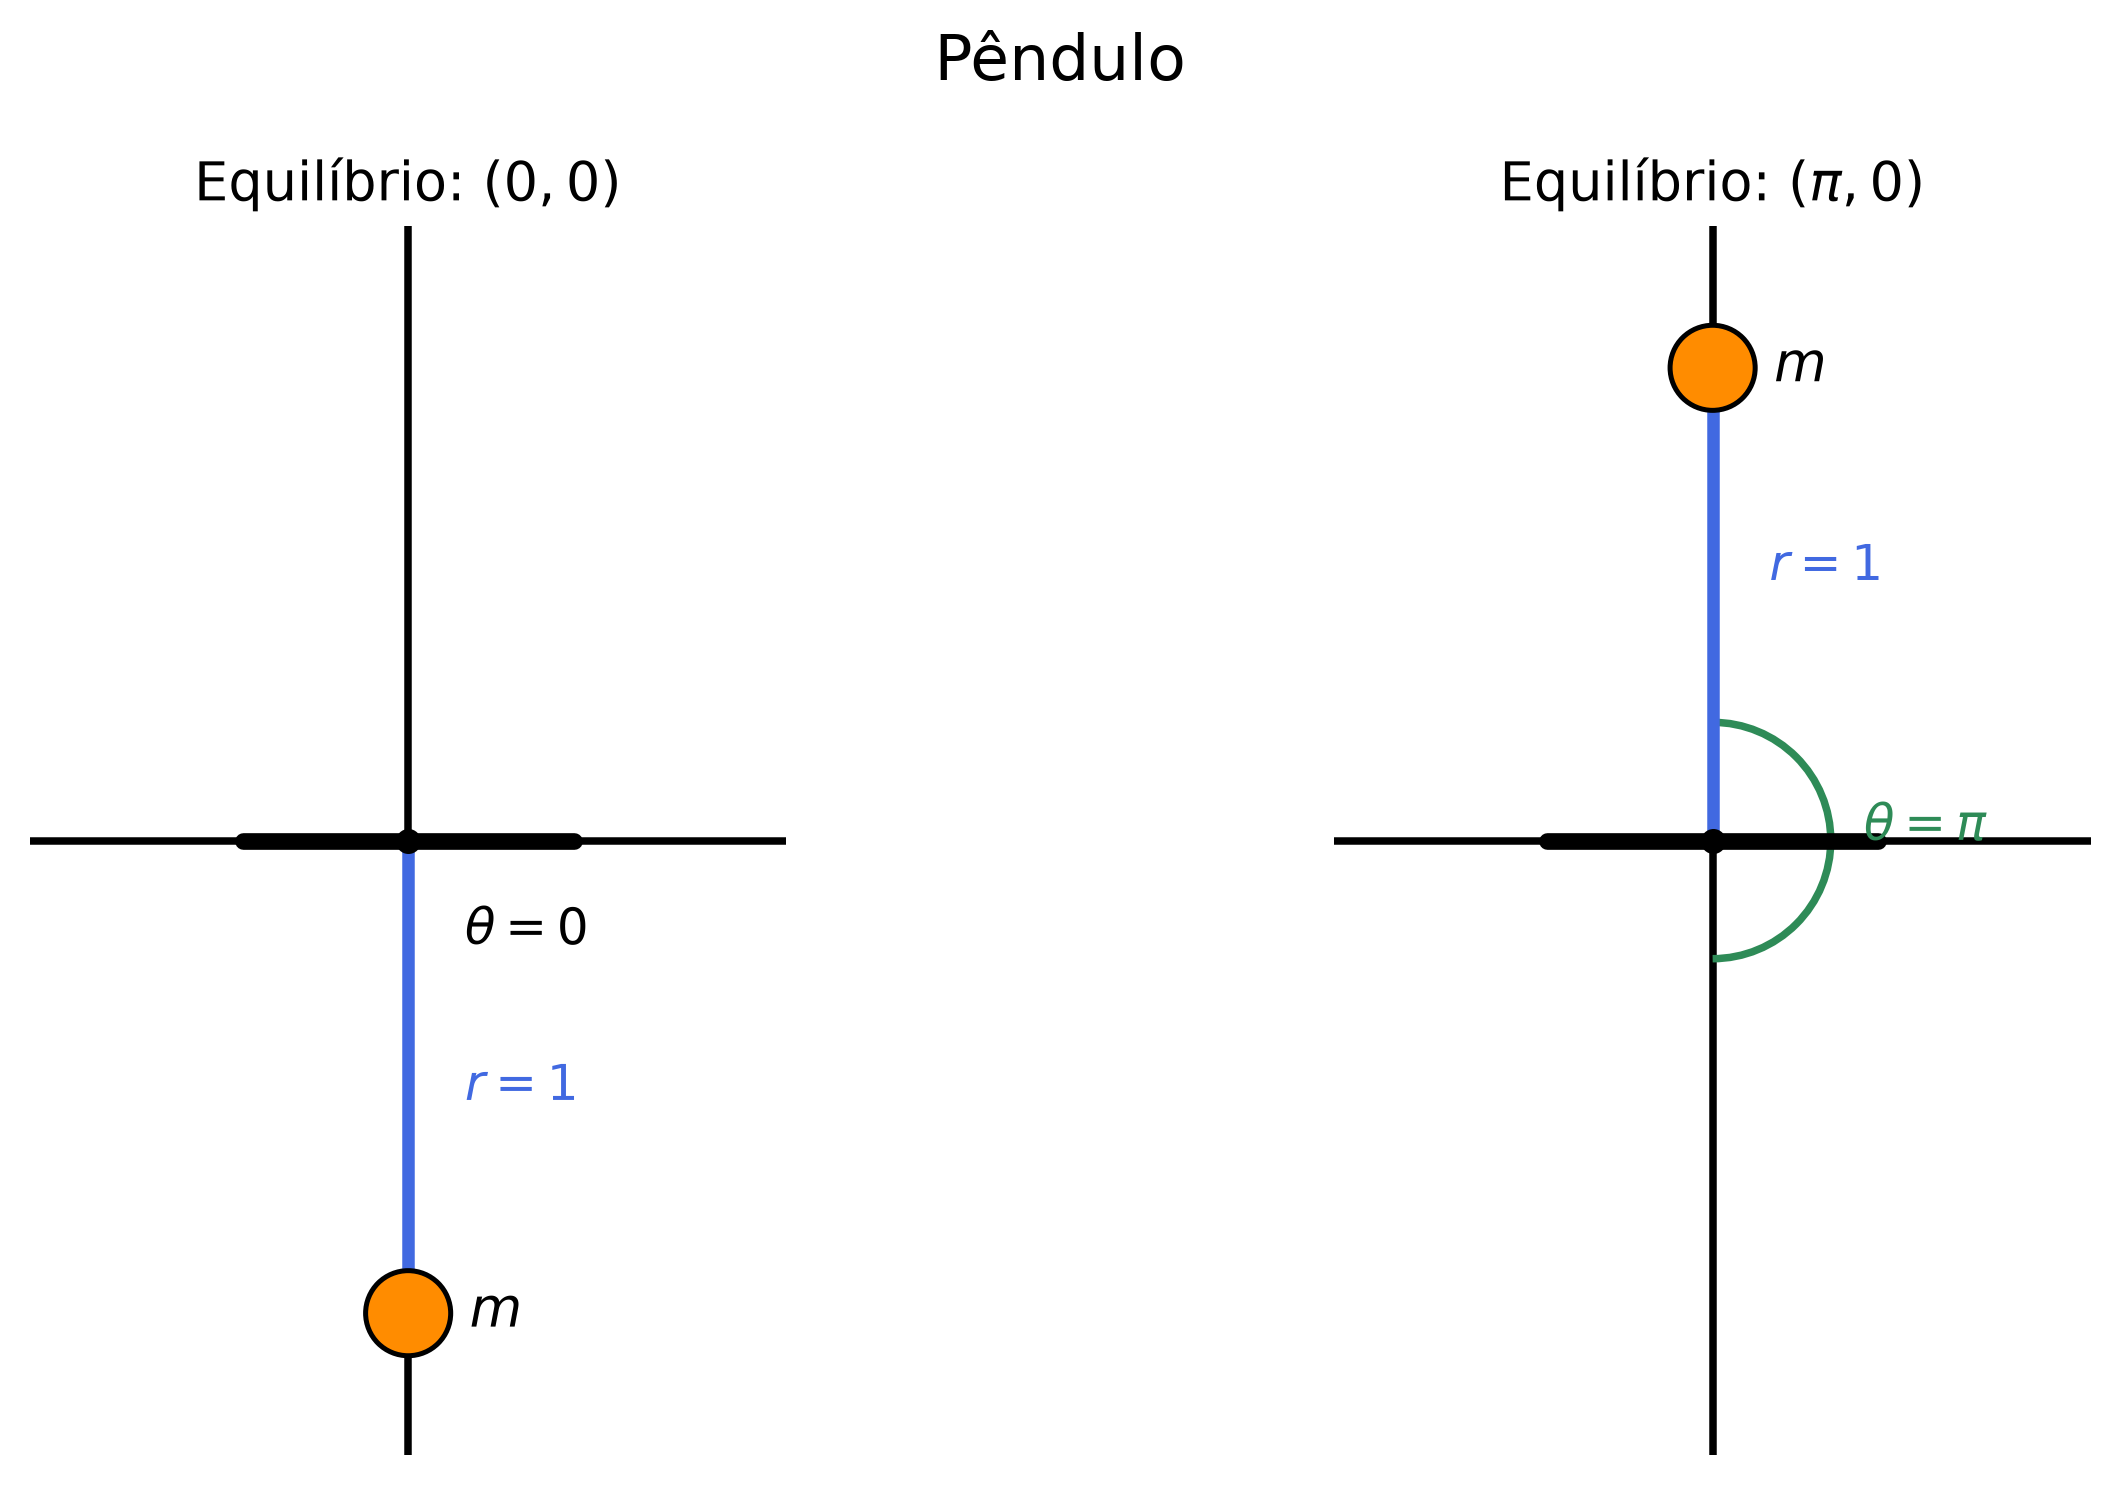
\includegraphics[scale=0.4]{figuras/pendulo.png}
  \end{center}
\end{frame}

\begin{frame}{}
  \begin{block}{}
    Vamos a estudar a linearização
    \begin{align*}
      Df(\theta,\omega)=\begin{pmatrix}
        0 & 1 \\
        -\cos(\theta) & -c
      \end{pmatrix}.
    \end{align*}
  \end{block}
\end{frame}

\begin{frame}{}
  Para $p_0=(0,0)$
    \begin{align*}
      A_0=Df(p_0)=\begin{pmatrix}
        0 & 1 \\
        -1 & -c
      \end{pmatrix},
    \end{align*}
    onde os autovalores são
    \begin{align*}
      \lambda_{\pm}=\frac{-c\pm\sqrt{c^2-4}}{2}.
    \end{align*}
    Neste caso, considerando $c>0$ temos que $Re \lambda_{\pm}<0$, pelo que temos que $p_0$ é um ponto singular hiperbólico. Portanto, usando o Teorema de Hartman-Grobman temos que existe $h:V\to W$ tal que
    \begin{align*}
      h(\phi_t(x))=e^{tA_0}h(x).
    \end{align*}
    Logo, podemos garantir que $p_0$ é uma singularidade assintoticamente estável no sistema não linear.\\
\end{frame}

\begin{frame}{}
  \begin{center}
  \begin{minipage}[c]{0.53\textwidth}
    \centering
    \animategraphics[
      width=\textwidth,
      autoplay,
      loop
    ]{20}{figuras/animacoes/linear_estavel/linear_estavel1_}{000}{001}
  \end{minipage}%
  \begin{minipage}[c]{0.53\textwidth}
    \centering
    \animategraphics[
      width=\textwidth,
      autoplay,
      loop
    ]{20}{figuras/animacoes/linear_nao_estavel/linear_nao_estavel1_}{000}{001}
  \end{minipage}
\end{center}

\end{frame}

\begin{frame}{}
  \begin{center}
  \begin{minipage}[c]{0.53\textwidth}
    \centering
    \animategraphics[
      width=\textwidth,
      autoplay,
      loop
    ]{20}{figuras/animacoes/pendulo_estavel/pendulo_}{000}{001}
  \end{minipage}%
  \begin{minipage}[c]{0.53\textwidth}
    \centering
    \animategraphics[
      width=\textwidth,
      autoplay,
      loop
    ]{20}{figuras/animacoes/pendulo_estavel/fase_}{000}{001}
  \end{minipage}
\end{center}

\end{frame}

\begin{frame}{}
  Para $p_1=(\pi,0)$
    \begin{align*}
      A_1=Df(p_0)=\begin{pmatrix}
        0 & 1 \\
        1 & -c
      \end{pmatrix},
    \end{align*}
    onde os autovalores são
    \begin{align*}
      \lambda_{\pm}=\frac{-c\pm\sqrt{c^2+4}}{2}.
    \end{align*}
    Neste caso, $c<\sqrt{c^{2}+4}$, logo temos que $\lambda_{+}>0$ e $\lambda_{-}<0$, pelo que temos que $p_1$ é um ponto singular hiperbólico. Portanto, usando o Teorema de Hartman-Grobman temos que existe $h:V\to W$ tal que
    \begin{align*}
      h(\phi_t(x))=e^{tA_0}h(x).
    \end{align*}
    Logo, podemos garantir que $p_1$ é uma singularidade instável no sistema não linear.
\end{frame}

\begin{frame}{}
  \begin{center}
  \begin{minipage}[c]{0.53\textwidth}
    \centering
    \animategraphics[
      width=\textwidth,
      autoplay,
      loop
    ]{20}{figuras/animacoes/linear_instavel/linear_instavel1_}{000}{001}
  \end{minipage}%
  \begin{minipage}[c]{0.53\textwidth}
    \centering
    \animategraphics[
      width=\textwidth,
      autoplay,
      loop
    ]{20}{figuras/animacoes/linear_nao_instavel/linear_nao_instavel1_}{000}{001}
  \end{minipage}
\end{center}

\end{frame}

\begin{frame}{}
  \begin{center}
  \begin{minipage}[c]{0.53\textwidth}
    \centering
    \animategraphics[
      width=\textwidth,
      autoplay,
      loop
    ]{20}{figuras/animacoes/pendulo_instavel/pendulo_}{000}{001}
  \end{minipage}%
  \begin{minipage}[c]{0.53\textwidth}
    \centering
    \animategraphics[
      width=\textwidth,
      autoplay,
      loop
    ]{20}{figuras/animacoes/pendulo_instavel/fase_}{000}{001}
  \end{minipage}
\end{center}

\end{frame}
